%-- einleitung

\section{Projektumsetzung}

\subsection{Programmiersprachen}

\subsection{Frameworks und Bibliotheken}

\subsection{Individuen und Populationen}

\begin{figure}[H]
\centering
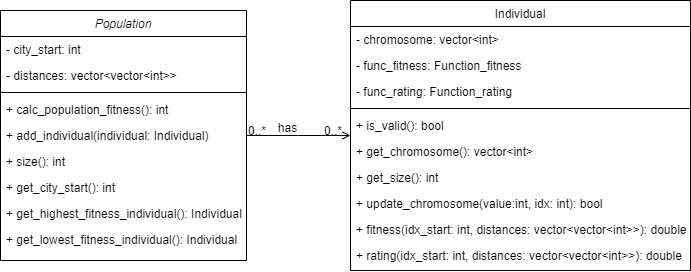
\includegraphics[width=1\textwidth]{img/Vortrag/uml.png}
\caption{Klassendiagramm Individuum und Population}
\label{fig:klassendiagramm}
\end{figure}


\subsection{Bewertungs und Fitnessfunktion}

\subsection{Marriage-Algorithmus}

\subsection{Crossover-Algorithmen}

\subsection{Mutations-Algorithmus}

\subsection{Selektions-Algorithmus}

\subsection{Simulator}

\begin{figure}[H]
\centering
\includegraphics[width=1\textwidth]{img/Vortrag/simulator.png}
\caption{Klassendiagramm Simulator}
\label{fig:simulator}
\end{figure}

\subsection{Python-Schnittstelle}

\subsection{Testen}

%--